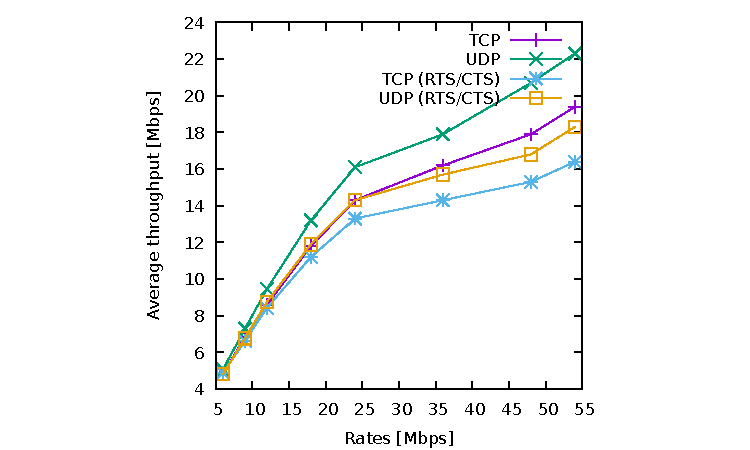
\includegraphics[width=0.5\textwidth]{traces/L3-3-1-tput.pdf}
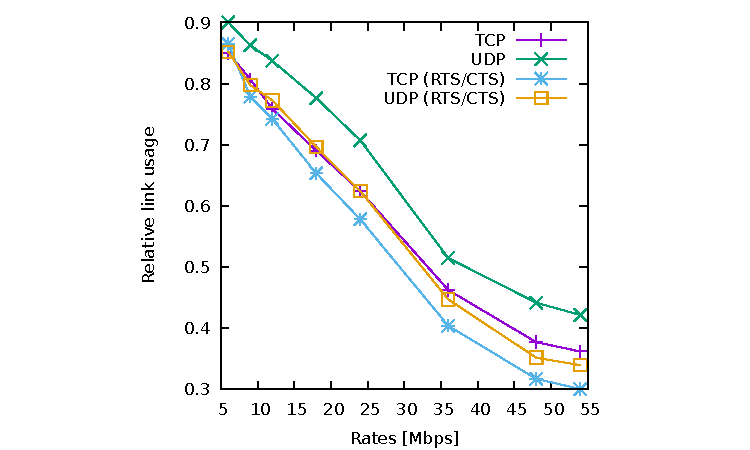
\includegraphics[width=0.5\textwidth]{traces/L3-3-1-usage.pdf}

For both TCP and UDP throughput is consistently lower with RTS/CTS enabled. Looking at the full iperf  output, we noticed UDP packet loss was, surprisingly, consistently higher with RTS/CTS enabled. Furthermore the RTS/CTS mechanism adds overhead, leading to lower throughput. \\ \\
Some additional research indicated that packets dropped before they are ever sent, are also counted towards packet loss. By analyzing the number of actually sent packets for UDP with tcpdump, we noticed all 'packet loss' was due to packets being dropped at the sender: every packet that was actually sent also arrived. Any time spent sending RTS/CTS packets could be considered 'wasted' in this case: there is no packet loss for it to prevent, and the time could have been spent sending additional data. Assuming there was no packet loss after transmission for TCP either, this explanation holds for TCP as well. \\ \\ Even with RTS/CTS enabled UDP still outperforms TCP: TCP's lower performance is caused by its additional overhead and congestion control, which is not changed by having RTS/CTS enabled.
